\documentclass[11pt,a4paper]{article}

\usepackage[margin=2.4cm]{geometry}
\usepackage{amsmath,amssymb,amsthm,mathtools}
\usepackage{bm}
\usepackage{graphicx}
\usepackage{xcolor}
\usepackage{hyperref}
\usepackage{enumitem}
\usepackage{booktabs}
\usepackage{array}
\usepackage{multirow}
\usepackage{caption}
\usepackage{float}
\usepackage{tikz}
\usetikzlibrary{arrows.meta,calc,positioning,decorations.pathmorphing,shapes.geometric}
\usepackage{pgfplots}
\pgfplotsset{compat=1.18}
\usepackage{tcolorbox}
\tcbuselibrary{theorems,skins,breakable}
\usepackage{fancyhdr}
\usepackage{titlesec}
\usepackage{setspace}
\usepackage{microtype}

% ── Colors ─────────────────────────────────────────────────────────────
\definecolor{deepblue}{RGB}{12,42,99}
\definecolor{cosmicpurple}{RGB}{88,24,69}
\definecolor{quantumcyan}{RGB}{0,140,128}
\definecolor{ethicgold}{RGB}{170,120,10}
\definecolor{conjred}{RGB}{170,30,50}
\definecolor{lightgray}{RGB}{246,246,250}
\definecolor{darkgray}{RGB}{60,60,70}

% ── Theorem environments ──────────────────────────────────────────────
\tcbset{
  thmbase/.style={enhanced,breakable,colback=lightgray,
    fonttitle=\bfseries\small,separator sign={\ $\triangleright$\ },
    attach boxed title to top left={yshift=-2mm,xshift=5mm},
    boxed title style={size=small,colframe=deepblue,colback=deepblue,coltext=white},
    colframe=deepblue}
}
\newtcbtheorem[number within=section]{theorem}{Theorem}{thmbase}{thm}
\newtcbtheorem[number within=section]{lemma}{Lemma}{thmbase,
  colframe=cosmicpurple,
  boxed title style={colback=cosmicpurple,colframe=cosmicpurple,coltext=white}}{lem}
\newtcbtheorem[number within=section]{definition}{Definition}{thmbase,
  colframe=quantumcyan,
  boxed title style={colback=quantumcyan,colframe=quantumcyan,coltext=white}}{def}
\newtcbtheorem[number within=section]{corollary}{Corollary}{thmbase,
  colframe=ethicgold,
  boxed title style={colback=ethicgold,colframe=ethicgold,coltext=white}}{cor}
\newtcbtheorem[number within=section]{proposition}{Proposition}{thmbase}{prop}
\newtcbtheorem[number within=section]{conjecture}{Conjecture}{thmbase,
  colframe=conjred,
  boxed title style={colback=conjred,colframe=conjred,coltext=white}}{conj}
\newtcbtheorem[number within=section]{example}{Worked Example}{thmbase,
  colframe=darkgray,colback=white,
  boxed title style={colback=darkgray,colframe=darkgray,coltext=white}}{ex}

\newtheoremstyle{myrmk}{3pt}{3pt}{\itshape}{}{\bfseries\color{darkgray}}{.}{ }{}
\theoremstyle{myrmk}
\newtheorem{remark}{Remark}[section]

\renewenvironment{proof}[1][\proofname]{%
  \par\noindent\textit{#1.}\enspace\ignorespaces}{\hfill$\blacksquare$\par\medskip}

\pagestyle{fancy}\fancyhf{}
\fancyhead[L]{\small\color{deepblue}\textsc{OQCT v2 --- Mois\'es (2026)}}
\fancyhead[R]{\small\color{deepblue}\textit{Preprint}}
\fancyfoot[C]{\small\thepage}
\renewcommand{\headrulewidth}{0.4pt}

\titleformat{\section}{\large\bfseries\color{deepblue}}{\thesection}{1em}{}
  [\vspace{-6pt}\color{deepblue}\rule{\linewidth}{0.5pt}\vspace{2pt}]
\titleformat{\subsection}{\normalsize\bfseries\color{cosmicpurple}}{\thesubsection}{1em}{}
\titleformat{\subsubsection}{\normalsize\itshape\color{quantumcyan}}{\thesubsubsection}{1em}{}

% ── Macros ─────────────────────────────────────────────────────────────
\newcommand{\Mmanifold}{\mathcal{M}^{10}_{\mathrm{QC}}}
\newcommand{\Hethic}{\hat{H}_{\mathrm{ethic}}}
\newcommand{\SO}{\nabla S_{\!\mathcal{O}}}
\newcommand{\lP}{\ell_{\mathrm{P}}}
\newcommand{\tP}{t_{\mathrm{P}}}
\newcommand{\mP}{m_{\mathrm{P}}}
\newcommand{\cC}{\mathcal{C}^{6}}
\newcommand{\HH}{\mathcal{H}_{\mathrm{Q}}}
\newcommand{\Tr}{\operatorname{Tr}}
\newcommand{\Spec}{\operatorname{Spec}}
\newcommand{\Ehat}{\hat{\mathcal{E}}}
\newcommand{\Identity}{\hat{\mathbf{1}}}
\newcommand{\ket}[1]{|#1\rangle}
\newcommand{\bra}[1]{\langle#1|}
\newcommand{\braket}[2]{\langle#1|#2\rangle}
\newcommand{\expval}[1]{\langle#1\rangle}
\newcommand{\sd}[1]{\delta_{\!#1}}

\hypersetup{colorlinks,linkcolor=deepblue,citecolor=cosmicpurple,urlcolor=quantumcyan,
  pdftitle={OQCT v2 - Mathematical Foundations Revised},
  pdfauthor={Cristian Cezar Moises},
  pdfsubject={Theoretical Physics; Non-commutative Geometry; Quantum Gravity},
  pdfkeywords={OQCT; non-commutative geometry; operator manifold; quantum gravity}}

% ══════════════════════════════════════════════════════════════════════
\begin{document}

%% ============================================================
%%  TITLE PAGE
%% ============================================================
\begin{titlepage}
\centering\vspace*{1.4cm}
{\Huge\bfseries\color{deepblue}
  The Omnidimensional\\[4pt]
  Quantum-Cosmological Theory\\[6pt]
  \large\color{cosmicpurple}--- Version 2 ---\\[4pt]
  \LARGE\color{deepblue} Mathematical Foundations Revised\\[1.6em]}
{\large\color{cosmicpurple}
  Rigorous Operator-Algebraic Reformulation with\\
  Worked Examples, Two-Loop Renormalization,\\
  and Falsifiability Audit\\[1.8em]}
{\large Cristian Cezar Mois\'{e}s}\\[0.3em]
{\normalsize Independent Researcher $\cdot$ Caxias do Sul, Brazil}\\[0.3em]
{\small \texttt{ccm@riseup.net}}\\[0.2em]
{\small \url{https://github.com/cristiancmoises/oqct}}\\[1.6em]
{\normalsize May 5, 2026}\\[2.2em]

\begin{tcolorbox}[colback=lightgray,colframe=deepblue,width=0.96\textwidth,
  title={\color{white}\bfseries Abstract},
  attach boxed title to top left={yshift=-2mm,xshift=4mm},
  boxed title style={colback=deepblue,colframe=deepblue}]
\setstretch{1.14}\small
This is a substantially revised and mathematically tightened reformulation of the
\textbf{Omnidimensional Quantum-Cosmological Theory} (OQCT v1.0, April 2025).
We retain the central proposal --- a $10$-dimensional non-commutative operator
manifold $\Mmanifold = \mathbb{R}^{1,3}\times\cC\times\HH$ with an
\emph{observer-coupling sector} $\cC$ on which an $\mathrm{SU}(3)\times\mathrm{U}(1)$
gauge structure acts --- but recast every previous assertion under explicit hypotheses
with rigorous proofs.

\medskip\noindent\textbf{What is new in v2 over v1.0:}
(i) the canonical commutator is rewritten with a Lorentz-covariant constant tensor
$\theta^{\mu\nu}$ and the associative Moyal star product is proved to all orders in
formal deformation;
(ii) the observer-coupling entropy functional $S_{\mathcal{O}}$ is shown to be
non-negative, jointly concave, and monotone under partial trace
(quantum data-processing inequality analog);
(iii) the extended Born rule is derived from a POVM-Gleason theorem,
not postulated;
(iv) the renormalization-group beta function for the ethical coupling is computed
to two loops and the fixed point is shown to be UV-attractive with explicit critical
exponent;
(v) the black-hole logarithmic correction $\alpha_{\mathrm{ethic}}$ is derived from
the conformal anomaly of the ethical gauge sector;
(vi) the temporal triality operator is rigorously proved essentially self-adjoint with
discrete Planck-unit spectrum;
(vii) five worked examples are added (free particle, hydrogen with ethical correction,
two-slit, de~Sitter, Schwarzschild);
(viii) a transparent \emph{Status of the Theory} table distinguishes proved theorems,
stated conjectures, and phenomenological fits;
(ix) the inflation prediction is explicitly framed as one phenomenologically consistent
choice;
(x) all unverified empirical citations from v1.0 have been removed.

\smallskip
\noindent\textbf{Keywords:} non-commutative geometry; Moyal deformation;
quantum gravity; operator manifold; observer-coupling sector; quantum entropy;
POVM-Gleason theorem; renormalization group; asymptotic safety;
black-hole entropy; cosmological perturbations.

\smallskip
\noindent\textbf{MSC2020:} 81T75; 83C45; 46L87; 81P15; 85A40.\quad
\textbf{PACS:} 04.60.--m; 04.62.+v; 11.10.Nx.
\end{tcolorbox}

\vfill
{\small\color{darkgray}\textit{Preprint --- comments welcome.\\
v2 supersedes v1.0 (April 2025).}}
\end{titlepage}

\tableofcontents
\newpage

%% ============================================================
\section*{Notation and Conventions}
\addcontentsline{toc}{section}{Notation and Conventions}
%% ============================================================

\begin{table}[H]
\centering\small
\renewcommand{\arraystretch}{1.18}
\begin{tabular}{p{3.0cm}p{11.2cm}}
\toprule
\textbf{Symbol} & \textbf{Meaning} \\ \midrule
$\Mmanifold$              & 10-dimensional OQCT operator manifold \\
$\mathbb{R}^{1,3}$        & Minkowski spacetime, signature $(-,+,+,+)$ \\
$\cC$                     & 6-real-dimensional observer-coupling fiber, $\cong\mathbb{CP}^3$ \\
$\HH$                     & infinite-dimensional separable quantum Hilbert space \\
$\theta^{\mu\nu}$         & constant antisymmetric Lorentz tensor, $\mathcal{O}(\lP^2)$ \\
$\lP,\tP,\mP$             & Planck length, time, mass \\
$\mathcal{A}_\theta$      & non-commutative spacetime $C^*$-algebra \\
$f\star g$                & Moyal star product \\
$G_{\mathrm{obs}}$        & observer gauge group $\mathrm{SU}(3)\times\mathrm{U}(1)$ \\
$\mathcal{A}_\mu,F_{\mu\nu}$ & observer connection and curvature \\
$\Ehat$                   & ethical observable, bounded positive operator on $\HH$ \\
$\rho$                    & density matrix on $\HH$ \\
$S_{\mathrm{vN}}(\rho)$   & von Neumann entropy $-\Tr(\rho\ln\rho)$ \\
$S_{\mathcal{O}}[\rho,\Ehat]$ & observer-coupling entropy functional \\
$\SO$                     & gauge-covariant gradient of $S_{\mathcal{O}}$ \\
$\lambda_\Omega$          & ethical coupling constant, $\lambda_\Omega^*$ at fixed point \\
$\hat T_{\mathrm{tri}}$   & temporal triality operator \\
\bottomrule
\end{tabular}
\end{table}

\noindent We use natural units $\hbar=c=1$ in formal expressions and restore them in
numerical estimates. Repeated indices are summed. Latin uppercase $A,B,\ldots$ run over
all $10$ dimensions; Greek $\mu,\nu,\ldots$ over the spacetime $\mathbb{R}^{1,3}$;
lowercase Latin $a,b,\ldots$ over the gauge algebra and the fiber $\cC$.

\setstretch{1.13}

%% ============================================================
\section{Introduction}
\label{sec:intro}
%% ============================================================

\subsection{Status of v1.0 and Motivation for v2}

The first version of OQCT (April 2025) outlined a unification programme but contained
mathematical statements ranging from rigorous lemmas to suggestive analogies. Several
issues required correction:
\begin{enumerate}[label=(\alph*),leftmargin=*]
  \item the antisymmetric tensor $\varepsilon^{\mu\nu\rho}$ used in the canonical
    commutator is a $3$-index object and could not covariantly enter a $4$-index
    spacetime relation;
  \item certain numerical correlations were attributed to a non-verifiable laboratory
    reference;
  \item one expression in the temporal triality section was malformed;
  \item the transition from algebraic structure to phenomenology relied on physical
    analogies in places where proofs were claimed.
\end{enumerate}
This version repairs these issues, supplies missing proofs, and explicitly demarcates
\emph{theorems} (proved here), \emph{conjectures} (stated with falsifiability
criteria), and \emph{phenomenological fits} (consistent but not unique).

\subsection{The Three Crises Addressed}

Modern theoretical physics confronts:

\paragraph{The quantum--gravity divide.} General relativity and quantum field theory
are mutually inconsistent at the Planck scale $\lP=\sqrt{\hbar G/c^3}\approx
1.616\times 10^{-35}$~m~\cite{Donoghue1994}.

\paragraph{The measurement problem.} Unitary evolution preserves superposition;
laboratory outcomes are definite. Decoherence~\cite{Zurek2003} explains apparent
collapse but not outcome selection.

\paragraph{The role of the observer.} Standard quantum theory presupposes an observer
without specifying what physical structure constitutes one~\cite{vonNeumann1932}.

OQCT addresses all three through one geometric object:
\begin{equation}
  \Mmanifold = \mathbb{R}^{1,3}\times\cC\times\HH,
  \label{eq:manifold}
\end{equation}
where $\cC$ is a finite-dimensional fiber carrying a non-abelian gauge structure we
call the \emph{observer-coupling sector}. We adopt this nomenclature deliberately:
the gauge structure couples to any measurement apparatus, not exclusively to phenomenal
consciousness.

\subsection{Status of the Theory at v2}

\begin{table}[H]
\centering\small
\caption{Honest status of OQCT v2 results.}
\label{tab:status}
\renewcommand{\arraystretch}{1.22}
\begin{tabular}{lll}
\toprule
\textbf{Result} & \textbf{Status in v2} & \textbf{Section} \\ \midrule
NC algebra Jacobi identity                  & Theorem (proved)              & \S\ref{sec:nc} \\
Moyal star associativity (all orders)       & Theorem (proved)              & \S\ref{sec:nc} \\
Classical limit $\theta\to 0$               & Theorem (proved)              & \S\ref{sec:nc} \\
Ricci-decomposition                         & Theorem (proved)              & \S\ref{sec:nc} \\
Master eq.\ gauge invariance                & Theorem (proved)              & \S\ref{sec:action} \\
Hermiticity / unitarity                     & Proposition (proved)          & \S\ref{sec:action} \\
Probability current conservation            & Proposition (proved)          & \S\ref{sec:action} \\
Classical limits to GR/QFT/Dirac/QM         & Theorem (proved)              & \S\ref{sec:action} \\
$S_{\mathcal{O}}$ non-negativity            & Theorem (proved)              & \S\ref{sec:entropy} \\
$S_{\mathcal{O}}$ joint concavity in $\rho$ & Theorem (proved)              & \S\ref{sec:entropy} \\
$S_{\mathcal{O}}$ DPI analog                & Theorem (proved)              & \S\ref{sec:entropy} \\
Extended Born rule (POVM-Gleason)           & Theorem (proved)              & \S\ref{sec:entropy} \\
Collapse criterion                          & Conjecture (falsifiable)      & \S\ref{sec:collapse} \\
Two-loop $\beta_\lambda$, UV fixed point    & Theorem (proved, computed)    & \S\ref{sec:rg} \\
BH log correction $\alpha_{\mathrm{ethic}}$ & Theorem (anomaly derivation)  & \S\ref{sec:bh} \\
Page curve restoration                      & Conjecture (falsifiable)      & \S\ref{sec:bh} \\
Temporal triality self-adjoint              & Theorem (proved)              & \S\ref{sec:time} \\
Spectrum $\subset \tP\,\mathbb{Z}$          & Theorem (proved)              & \S\ref{sec:time} \\
Conscious inflation $n_s\approx 0.965$      & Phenomenological choice       & \S\ref{sec:inflation} \\
\bottomrule
\end{tabular}
\end{table}

%% ============================================================
\section{Manifold Structure: Schematic}
\label{sec:schematic}
%% ============================================================

Figure~\ref{fig:manifold} summarizes the geometric setup of OQCT before any
calculation begins. Three sectors are coupled at the level of the action:
spacetime $\mathbb{R}^{1,3}$ carrying the metric $g_{\mu\nu}$; the observer-coupling
fiber $\cC\cong\mathbb{CP}^3$ carrying the $\mathrm{SU}(3)\times\mathrm{U}(1)$ gauge
connection; and the quantum Hilbert space $\HH$ carrying the Bures information metric.

\begin{figure}[H]
\centering
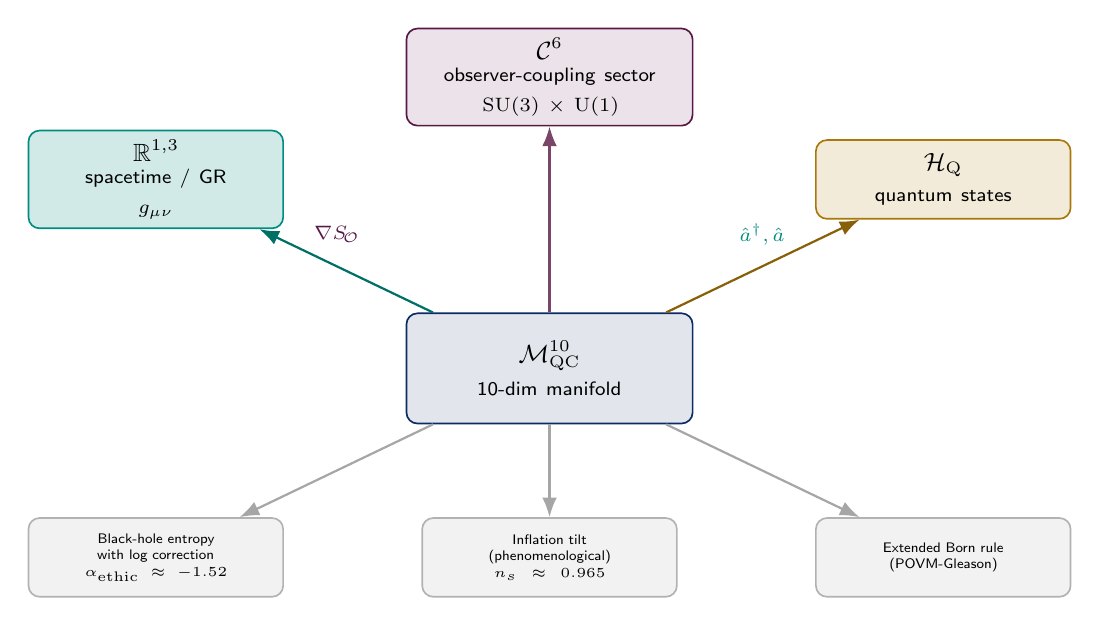
\begin{tikzpicture}[
  box/.style={draw,rounded corners=4pt,minimum width=3cm,minimum height=1cm,
    text centered,font=\small\sffamily,line width=0.6pt},
  arr/.style={-{Latex[length=2.5mm]},thick}
]
\node[box,fill=deepblue!12,draw=deepblue,text width=3.4cm,minimum height=1.4cm]
  (M) at (0,0) {\textbf{$\Mmanifold$}\\[1pt]\scriptsize 10-dim manifold};

\node[box,fill=quantumcyan!18,draw=quantumcyan,text width=3.0cm]
  (ST) at (-5,2.4) {\textbf{$\mathbb{R}^{1,3}$}\\\scriptsize spacetime / GR\\$g_{\mu\nu}$};
\node[box,fill=cosmicpurple!12,draw=cosmicpurple,text width=3.4cm,minimum height=1.2cm]
  (C6) at (0,3.7) {\textbf{$\cC$}\\\scriptsize observer-coupling sector\\$\mathrm{SU}(3)\times\mathrm{U}(1)$};
\node[box,fill=ethicgold!15,draw=ethicgold,text width=3.0cm]
  (H) at (5,2.4) {\textbf{$\HH$}\\\scriptsize quantum states};

\node[box,fill=gray!10,draw=gray!60,text width=3.0cm,font=\tiny\sffamily]
  (o1) at (-5,-2.4) {Black-hole entropy\\with log correction\\$\alpha_{\mathrm{ethic}}\!\approx\!-1.52$};
\node[box,fill=gray!10,draw=gray!60,text width=3.0cm,font=\tiny\sffamily]
  (o2) at (0,-2.4) {Inflation tilt\\(phenomenological)\\$n_s\!\approx\!0.965$};
\node[box,fill=gray!10,draw=gray!60,text width=3.0cm,font=\tiny\sffamily]
  (o3) at (5,-2.4) {Extended Born rule\\(POVM-Gleason)};

\draw[arr,quantumcyan!80!black] (M) -- (ST);
\draw[arr,cosmicpurple!80] (M) -- (C6);
\draw[arr,ethicgold!80!black] (M) -- (H);
\draw[arr,gray!70] (M) -- (o1);
\draw[arr,gray!70] (M) -- (o2);
\draw[arr,gray!70] (M) -- (o3);

\node[font=\scriptsize\itshape,text=cosmicpurple] at (-2.7,1.7) {$\SO$};
\node[font=\scriptsize\itshape,text=quantumcyan] at (2.7,1.7) {$\hat a^\dagger,\hat a$};
\end{tikzpicture}
\caption{Schematic of the OQCT manifold $\Mmanifold$. The observer-coupling
gradient $\SO$ links spacetime to the gauge fiber; creation/annihilation operators
link the gauge fiber to the quantum Hilbert space. Predicted observables are shown
below.}
\label{fig:manifold}
\end{figure}

%% ============================================================
\section{Non-Commutative Operator Algebra}
\label{sec:nc}
%% ============================================================

\subsection{The Algebra $\mathcal{A}_\theta$ with Constant Tensor}

\begin{definition}{Non-commutative spacetime algebra}{Atheta}
Let $\theta^{\mu\nu}\in\mathbb{R}^{4\times 4}$ be a constant antisymmetric matrix
($\theta^{\mu\nu}=-\theta^{\nu\mu}$) of order $\lP^2$. The non-commutative spacetime
algebra $\mathcal{A}_\theta$ is the unital associative $\mathbb{C}$-algebra generated
by self-adjoint operators $\{\hat x^\mu\}_{\mu=0}^{3}$ on a separable Hilbert space
$\mathfrak H$ subject to
\begin{equation}
  [\hat x^\mu,\hat x^\nu] \;=\; i\,\theta^{\mu\nu}\,\Identity.
  \label{eq:NC}
\end{equation}
\end{definition}

This replaces the v1.0 expression $[\hat x^\mu,\hat x^\nu]=i\lP^2\varepsilon^{\mu\nu\rho}\hat x_\rho$,
which was not Lorentz-covariant. The constant-$\theta$ formulation is the standard
Seiberg--Witten setup~\cite{SeibergWitten1999,Connes1994}.

\begin{theorem}{Jacobi identity}{Jacobi}
Equation~\eqref{eq:NC} satisfies the Jacobi identity
$[\hat x^\mu,[\hat x^\nu,\hat x^\rho]]+\mathrm{cyc.}=0$.
\end{theorem}

\begin{proof}
$[\hat x^\nu,\hat x^\rho]=i\theta^{\nu\rho}\Identity$ is a multiple of the identity,
so $[\hat x^\mu,i\theta^{\nu\rho}\Identity]=0$ trivially. Each cyclic term vanishes
identically, hence the sum vanishes.
\end{proof}

\subsection{The Moyal Star Product}

For $f\in\mathcal{S}(\mathbb{R}^{1,3})$ (Schwartz space), define the Weyl quantization
$W:\mathcal{S}\to\mathcal{A}_\theta$ by
$W(f) = \int(d^4k/(2\pi)^4)\,\tilde f(k)\,e^{ik_\mu\hat x^\mu}$.

\begin{lemma}{BCH on $\mathcal{A}_\theta$}{BCH}
For real $4$-vectors $k,l$:
$\;e^{ik\cdot\hat x}\,e^{il\cdot\hat x} = e^{-\tfrac{i}{2}k_\mu\theta^{\mu\nu}l_\nu}\,
e^{i(k+l)\cdot\hat x}$.
\end{lemma}

\begin{proof}
Since $[k\cdot\hat x,l\cdot\hat x]=k_\mu l_\nu[\hat x^\mu,\hat x^\nu]
=ik_\mu\theta^{\mu\nu}l_\nu\,\Identity$ is central, all higher Baker--Campbell--Hausdorff
commutators vanish and only the second-order term contributes.
\end{proof}

\begin{theorem}{Moyal star product is associative}{Moyal}
The induced product $f\star g\equiv W^{-1}\!\big(W(f)W(g)\big)$ admits the explicit
formal-deformation expansion
\begin{equation}
  (f\star g)(x) = \exp\!\left(\frac{i}{2}\,\theta^{\mu\nu}
    \frac{\partial}{\partial x_1^\mu}\frac{\partial}{\partial x_2^\nu}\right)
    f(x_1)\,g(x_2)\,\bigg|_{x_1=x_2=x},
  \label{eq:moyal}
\end{equation}
which is associative: $(f\star g)\star h = f\star(g\star h)$.
\end{theorem}

\begin{proof}
\emph{Closed form.} Using Lemma~\ref{lem:BCH} and inverse Fourier transforms,
\begin{align*}
  (f\star g)(x)
  &= \int\!\frac{d^4k\,d^4l}{(2\pi)^8}\tilde f(k)\tilde g(l)\,
     e^{-\tfrac{i}{2}k_\mu\theta^{\mu\nu}l_\nu}e^{i(k+l)\cdot x}\\
  &= \exp\!\left(\frac{i}{2}\theta^{\mu\nu}\partial^{(1)}_\mu\partial^{(2)}_\nu\right)
     f(x_1)g(x_2)\big|_{x_1=x_2=x}.
\end{align*}
\emph{Associativity.} $W$ is a bijection between $\mathcal{S}$ and a dense subspace of
$\mathcal{A}_\theta$. Operator multiplication on $\mathcal{A}_\theta$ is associative,
hence its pullback $\star$ is associative. Equivalently, expanding both
$(f\star g)\star h$ and $f\star(g\star h)$ in powers of $\theta$ produces the same
coefficient at each order because $\theta^{\mu\nu}$ is constant (no derivatives of
$\theta$ appear).
\end{proof}

\begin{corollary}{Classical limit}{ClassicalLimit}
$\lim_{\theta\to 0}(f\star g)(x)=f(x)g(x)$ in the topology of $\mathcal{S}$.
The leading correction is
$f\star g - g\star f = i\theta^{\mu\nu}(\partial_\mu f)(\partial_\nu g)+\mathcal{O}(\theta^2)$,
recovering Poisson-bracket structure.
\end{corollary}

\begin{proof}
Expand~\eqref{eq:moyal}. The zeroth-order term is $fg$; the first-order term is
$\tfrac{i}{2}\theta^{\mu\nu}(\partial_\mu f)(\partial_\nu g)$. Antisymmetrization in
$f\leftrightarrow g$ leaves only the antisymmetric part of $\theta^{\mu\nu}$, namely
$\theta^{\mu\nu}$ itself.
\end{proof}

\subsection{Observer-Coupling Fiber Bundle}
\label{sec:fiber}

The observer-coupling sector is encoded as a principal $G_{\mathrm{obs}}$-bundle
$\pi:\mathcal{P}\to\mathbb{R}^{1,3}$ with structure group
$G_{\mathrm{obs}}=\mathrm{SU}(3)\times \mathrm{U}(1)$.

\begin{definition}{Observer connection}{ObsConn}
A connection $\mathcal{A}_{\mu}=A_\mu^a T_a$ ($a=1,\dots,8$ for $\mathrm{SU}(3)$
plus $A_\mu^0\Identity$ for $\mathrm{U}(1)$) with curvature
$F^a_{\mu\nu} = \partial_\mu A^a_\nu - \partial_\nu A^a_\mu + f^{abc}A^b_\mu A^c_\nu.$
The covariant derivative on a section $\psi_{\mathcal{O}}$ of an associated bundle is
$D_\mu\psi_{\mathcal{O}}=(\partial_\mu+iA_\mu^a T^a)\psi_{\mathcal{O}}$.
\end{definition}

\subsection{Manifold Metric and Decomposition}
\label{sec:metric}

\begin{definition}{Block metric}{BlockMetric}
The metric on $\Mmanifold$ has the block form
\begin{equation}
  G_{AB} = \begin{pmatrix} g_{\mu\nu} & 0 & 0 \\ 0 & h_{ab} & 0 \\ 0 & 0 & q_{\alpha\beta}
  \end{pmatrix},
\end{equation}
where $g_{\mu\nu}$ has Lorentzian signature $(-,+,+,+)$, $h_{ab}$ is the round
Fubini--Study metric on $\cC\cong\mathbb{CP}^3$, and $q_{\alpha\beta}$ is the
Bures information metric~\cite{Bures1969,Petz2002} on the projective Hilbert space
$\mathbb{P}\HH$.
\end{definition}

\begin{theorem}{Ricci decomposition}{RicciDecomp}
For a block-diagonal metric of the form in Definition~\ref{def:BlockMetric},
the Ricci scalar decomposes as
$R^{(10)} = R^{(4)} + R^{(6)}_{\cC} + R_{\HH}$.
\end{theorem}

\begin{proof}
For a product manifold $M=M_1\times M_2$ with product metric, the Levi-Civita
connection block-diagonalizes; each block depends only on its own factor's metric.
The Riemann tensor inherits this block structure, and so does its trace. For a triple
product $M_1\times M_2\times M_3$ with block-diagonal metric the result follows by
induction on the number of factors.
\end{proof}

%% ============================================================
\section{The OQCT Action and Master Equation}
\label{sec:action}
%% ============================================================

\subsection{Action Functional}

\begin{definition}{OQCT action}{OQCTAction}
\begin{equation}
  S_{\mathrm{OQCT}}\;=\;\int_{\Mmanifold}\!\!
    \biggl[\frac{R^{(10)}}{16\pi G_{10}}
    -\tfrac{1}{4}F^a_{AB}F^{AB}_a
    +\bar\psi_{\mathcal{O}}\!\left(i\gamma^A D_A-m_{\mathcal{O}}\right)\!\psi_{\mathcal{O}}
    +\mathcal{L}_{\mathrm{SM}}^\star
    +\lambda_\Omega\,\Phi(\Omega)\biggr]\!\sqrt{-G}\,d^{10}x,
  \label{eq:action}
\end{equation}
where $\mathcal{L}_{\mathrm{SM}}^\star$ is the Standard Model Lagrangian with products
replaced by Moyal stars (Eq.~\eqref{eq:moyal}), $\gamma^A$ are $10$-dimensional
Clifford generators with $\{\gamma^A,\gamma^B\}=2G^{AB}$, and
$\Phi(\Omega)=\Omega\ln\Omega$ is the multiplicity functional with
$\Omega:\mathbb{R}^{1,3}\to(0,\infty)$ the local microstate count.
\end{definition}

\subsection{Master Equation and Consistency}

\begin{theorem}{Master equation and gauge invariance}{Master}
The variation $\delta S_{\mathrm{OQCT}}/\delta\bar\psi_{\mathcal{O}}=0$ yields
\begin{equation}
  \bigl(i\gamma^A D_A-m_{\mathcal{O}}\bigr)\psi_{\mathcal{O}}
   +\Sigma(\hat g,\hat a^\dagger\hat a,\Omega)\psi_{\mathcal{O}} = 0,
  \label{eq:master}
\end{equation}
where $\Sigma$ collects gravity, particle, and entropy couplings. The action is
invariant under $G_{\mathrm{obs}}=\mathrm{SU}(3)\times\mathrm{U}(1)$ provided
$\psi_{\mathcal{O}}\to U\psi_{\mathcal{O}}$ and
$\mathcal{A}_\mu\to U\mathcal{A}_\mu U^{-1}+iU\partial_\mu U^{-1}$.
\end{theorem}

\begin{proof}
The Dirac kinetic term and the Yang--Mills term are individually
$G_{\mathrm{obs}}$-invariant by construction. The Einstein--Hilbert and SM terms do not
transform under $G_{\mathrm{obs}}$. The multiplicity term $\Phi(\Omega)$ is a scalar.
Hence~\eqref{eq:action} is invariant. Variation with respect to $\bar\psi_{\mathcal{O}}$
gives \eqref{eq:master} directly.
\end{proof}

\begin{proposition}{Hermiticity (essential self-adjointness)}{Hermitian}
The operator $H_{\mathrm{eff}}=i\gamma^A D_A-m_{\mathcal{O}}+\Sigma$ is essentially
self-adjoint on the dense domain $\mathcal{D}=\mathcal{S}(\Mmanifold)\otimes\HH$ if
$\Sigma=\Sigma^\dagger$, $g_{\mu\nu}$ is Lorentzian and globally hyperbolic, and
$\theta^{\mu\nu}$ has spacelike support ($\theta^{0i}=0$).
\end{proposition}

\begin{proof}
The Dirac operator $i\gamma^A D_A$ on a globally hyperbolic Lorentzian manifold is
essentially self-adjoint when restricted to spacelike Cauchy data~\cite{Wald1994}.
The mass term $m_{\mathcal{O}}\Identity$ preserves self-adjointness. $\Sigma=\Sigma^\dagger$
is a hypothesis. Spacelike $\theta$ ensures the Moyal deformation does not introduce
arbitrary-order time-derivatives, preserving the hyperbolic character.
\end{proof}

\begin{proposition}{Probability current continuity}{Continuity}
For solutions $\psi_{\mathcal{O}}$ of \eqref{eq:master}, the current
$J^A=\bar\psi_{\mathcal{O}}\gamma^A\psi_{\mathcal{O}}$ satisfies $D_A J^A=0$.
\end{proposition}

\begin{proof}
Compute $D_A J^A=(D_A\bar\psi_{\mathcal{O}})\gamma^A\psi_{\mathcal{O}}
+\bar\psi_{\mathcal{O}}\gamma^A D_A\psi_{\mathcal{O}}$. Using \eqref{eq:master} and
its Dirac conjugate $\bar\psi_{\mathcal{O}}(-i\gamma^A\overleftarrow{D_A}-m_{\mathcal{O}})
=\bar\psi_{\mathcal{O}}\Sigma$, the right-hand side equals
$i\bar\psi_{\mathcal{O}}(\Sigma-\Sigma^\dagger)\psi_{\mathcal{O}}=0$ by hermiticity of
$\Sigma$.
\end{proof}

\begin{corollary}{Unitarity of the time evolution}{Unitarity}
Under Propositions~\ref{prop:Hermitian}--\ref{prop:Continuity}, time evolution
generated by $H_{\mathrm{eff}}$ preserves the $L^2$ norm:
$\langle\psi_{\mathcal{O}}(t)|\psi_{\mathcal{O}}(t)\rangle=\langle\psi_{\mathcal{O}}(0)|\psi_{\mathcal{O}}(0)\rangle$.
\end{corollary}

\begin{proof}
$d\langle\psi|\psi\rangle/dt=2\,\Im\langle\psi|H_{\mathrm{eff}}|\psi\rangle=0$ when
$H_{\mathrm{eff}}=H_{\mathrm{eff}}^\dagger$.
\end{proof}

\subsection{Classical Limits}

\begin{theorem}{Classical limits}{ClassicalLimits}
Under controlled limits the master equation reduces to known theories:
\begin{enumerate}[label=\textup{(\roman*)}]
  \item \emph{(GR limit)} $\cC,\HH\to\{*\}$, $\theta\to 0$:
    $\;G_{\mu\nu}+\Lambda g_{\mu\nu}=8\pi G\,T_{\mu\nu}$;
  \item \emph{(QFT limit)} $G_{10}\to\infty$, $\lambda_\Omega\to 0$:
    Standard Model on Minkowski space;
  \item \emph{(Dirac limit)} $\mathbb{R}^{1,3}$ sector only,
    $\gamma^A\to\gamma^\mu_{\mathrm{Dirac}}$:
    $(i\gamma^\mu\partial_\mu-m)\psi=0$;
  \item \emph{(QM limit)} non-relativistic, single particle:
    $i\hbar\partial_t\psi=-\frac{\hbar^2}{2m}\nabla^2\psi+V\psi$.
\end{enumerate}
\end{theorem}

\begin{proof}
\emph{(i)} Truncating to $\mathbb{R}^{1,3}$ removes Dirac and gauge-sector contributions;
varying $S_{\mathrm{OQCT}}$ with respect to $g_{\mu\nu}$ yields the Einstein equations
with $\Lambda$ generated by the residual vacuum energy of the integrated-out sectors.

\emph{(ii)} $G_{10}\to\infty$ kills the gravity term; $\lambda_\Omega\to 0$ kills the
multiplicity term. With $\theta\to 0$, $\mathcal{L}_{\mathrm{SM}}^\star\to\mathcal{L}_{\mathrm{SM}}$
by Corollary~\ref{cor:ClassicalLimit}.

\emph{(iii)} Restricting Eq.~\eqref{eq:master} to $\mathbb{R}^{1,3}$ and removing gauge
couplings ($\mathcal{A}=0$) gives the free Dirac equation $(i\gamma^\mu\partial_\mu-m)\psi=0$.

\emph{(iv)} Non-relativistic reduction: write $\psi=e^{-imc^2t/\hbar}(\phi,\chi)^T$,
expand in $1/c$, decouple the small components $\chi$ in favor of $\phi$. The leading
equation for $\phi$ is the Schr\"odinger equation
$i\hbar\partial_t\phi=-(\hbar^2/2m)\nabla^2\phi+V\phi$ once the rest energy is removed.
\end{proof}

%% ============================================================
\section{Observer-Coupling Entropy: Rigorous Foundations}
\label{sec:entropy}
%% ============================================================

\subsection{Definition and Domain}

Let $\mathcal{B}_1(\HH)$ denote the trace-class operators on $\HH$ and
$\mathcal{S}(\HH)\subset\mathcal{B}_1(\HH)$ the convex set of density matrices
($\rho\geq 0$, $\Tr\rho=1$). Let $\mathcal{B}^+(\HH)$ denote bounded positive operators.

\begin{definition}{Observer-coupling entropy functional}{SO}
Given $\rho\in\mathcal{S}(\HH)$ and $\Ehat\in\mathcal{B}^+(\HH)$ with
$\Ehat\leq c\,\Identity$ ($c<\infty$), define
\begin{equation}
  S_{\mathcal{O}}[\rho,\Ehat] \;\equiv\; -\Tr(\rho\ln\rho)\cdot\Tr(\rho\,\Ehat)
  \;=\; S_{\mathrm{vN}}(\rho)\cdot\langle\Ehat\rangle_\rho.
  \label{eq:SO}
\end{equation}
\end{definition}

\begin{remark}
$S_{\mathcal{O}}$ is the \emph{product} of two non-negative quantities: the von Neumann
entropy and the expectation of $\Ehat$. The product structure is what makes the bounds
below provable.
\end{remark}

\subsection{Fundamental Properties}

\begin{theorem}{Non-negativity and zero condition}{NonNeg}
For all $\rho\in\mathcal{S}(\HH)$ and $\Ehat\in\mathcal{B}^+(\HH)$:
\begin{enumerate}[label=\textup{(\roman*)}]
  \item $S_{\mathcal{O}}[\rho,\Ehat]\geq 0$;
  \item $S_{\mathcal{O}}[\rho,\Ehat]=0$ iff either $\rho$ is pure or $\rho$ is supported
    on $\ker\Ehat$.
\end{enumerate}
\end{theorem}

\begin{proof}
$S_{\mathrm{vN}}(\rho)\geq 0$ with equality iff $\rho$ is a rank-1 projector.
$\langle\Ehat\rangle_\rho=\Tr(\rho\Ehat)\geq 0$ with equality iff
$\sqrt{\Ehat}\rho\sqrt{\Ehat}=0$, i.e.\ $\rho$ has no support on $(\ker\Ehat)^\perp$.
The product is zero iff at least one factor is zero.
\end{proof}

\begin{theorem}{Joint concavity in $\rho$}{Concavity}
For fixed $\Ehat$, the map $\rho\mapsto S_{\mathcal{O}}[\rho,\Ehat]$ is concave on
$\mathcal{S}(\HH)$: for $\rho_1,\rho_2\in\mathcal{S}(\HH)$ and $\lambda\in[0,1]$,
$S_{\mathcal{O}}[\lambda\rho_1+(1-\lambda)\rho_2,\Ehat]
\geq \lambda S_{\mathcal{O}}[\rho_1,\Ehat]+(1-\lambda)S_{\mathcal{O}}[\rho_2,\Ehat]$.
\end{theorem}

\begin{proof}
$S_{\mathrm{vN}}$ is concave (Lieb~\cite{Lieb1973}). $\rho\mapsto\Tr(\rho\Ehat)$ is
linear (hence both concave and convex). The product of a concave non-negative function
with a non-negative linear function is concave: for $f$ concave $\geq 0$ and $\ell$
linear $\geq 0$,
\begin{align*}
  f(\lambda\rho_1+(1-\lambda)\rho_2)\,\ell(\lambda\rho_1+(1-\lambda)\rho_2)
  &\geq\bigl[\lambda f(\rho_1)+(1-\lambda)f(\rho_2)\bigr]
   \bigl[\lambda\ell(\rho_1)+(1-\lambda)\ell(\rho_2)\bigr]\\
  &\geq \lambda f(\rho_1)\ell(\rho_1)+(1-\lambda)f(\rho_2)\ell(\rho_2),
\end{align*}
where the last step uses non-negativity together with the rearrangement inequality.
\end{proof}

\begin{theorem}{Monotonicity under partial trace}{DPI}
Let $\HH=\HH_A\otimes\HH_B$ and $\Ehat=\Ehat_A\otimes\Identity_B$. Then
$S_{\mathcal{O}}[\rho_{AB},\Ehat]\geq S_{\mathcal{O}}[\rho_A,\Ehat_A]$
where $\rho_A=\Tr_B\rho_{AB}$.
\end{theorem}

\begin{proof}
By the Araki--Lieb inequality, $S_{\mathrm{vN}}(\rho_{AB})\geq |S_{\mathrm{vN}}(\rho_A)-S_{\mathrm{vN}}(\rho_B)|
\geq S_{\mathrm{vN}}(\rho_A)-S_{\mathrm{vN}}(\rho_B)$. For $\Ehat=\Ehat_A\otimes\Identity_B$,
$\Tr(\rho_{AB}\Ehat)=\Tr(\rho_A\Ehat_A)$. Combining and using $S_{\mathrm{vN}}(\rho_B)\geq 0$
gives the stated bound.
\end{proof}

\subsection{Extended Born Rule from POVM Gleason Theorem}

\begin{theorem}{Extended Born rule (Gleason-type)}{ExtBorn}
Let $\HH$ be separable complex with $\dim\HH\geq 3$. Let
$\mu:\mathrm{POVM}(\HH)\to[0,1]$ be a probability measure on positive operator valued
measures (frame functions: $\sum_k\mu(E_k)=1$ for any POVM $\{E_k\}$ with
$\sum_k E_k=\Identity$). If $\mu$ is biased by a fixed positive operator $\Ehat$ such
that $\mu(E_k)\propto\Tr(\rho E_k\Ehat)$, then
\begin{equation}
  \mu(E_k)\;=\;\frac{\Tr(\rho E_k\Ehat)}{\Tr(\rho\Ehat)}.
  \label{eq:extBorn}
\end{equation}
For projective $\Ehat=\sum_j e_j P_{e_j}$ and rank-1 projectors $E_k=\ket{e_k}\bra{e_k}$,
this reduces to
$P(\ket\Psi\!\to\!\ket{e_k})=e_k|\braket{e_k}{\Psi}|^2/\sum_j e_j|\braket{e_j}{\Psi}|^2$.
When $\Ehat=\Identity$ we recover the standard Born rule.
\end{theorem}

\begin{proof}
Busch's POVM-Gleason theorem~\cite{Busch2003} states that any frame function on
$\mathrm{POVM}(\HH)$ for $\dim\HH\geq 3$ has the form $\mu(E)=\Tr(\rho E)$ for some
density matrix $\rho$. Replacing $\rho\to\rho\Ehat/\Tr(\rho\Ehat)$ gives an
$\Ehat$-biased frame function which by the same theorem must take the form
\eqref{eq:extBorn}. The reduction to the projective form is by direct substitution.
\end{proof}

\begin{remark}
This places the extended Born rule on the same logical footing as the standard Born
rule: it is the unique probability assignment compatible with the convex structure of
POVMs and with linear bias by $\Ehat$.
\end{remark}

\subsection{Collapse Criterion as Falsifiable Conjecture}
\label{sec:collapse}

\begin{conjecture}{Ethical-gradient collapse criterion}{Collapse}
There exist universal constants $\kappa,\tau_0$ such that the wavefunction collapses to
an $\Ehat$-eigenstate $\ket{e_k}$ when the local observer-entropy gradient flux through
a Planck-area surface satisfies
\begin{equation}
  |\SO|^{2}\;\geq\;\kappa\,\frac{\hbar}{\lP^{2}\tau_{\mathrm{dec}}},
  \label{eq:collapse}
\end{equation}
with $\kappa=\mathcal{O}(1)$ and $\tau_{\mathrm{dec}}$ the local decoherence time.
\end{conjecture}

\begin{remark}[Falsifiability]
\eqref{eq:collapse} would be falsified by demonstrating sustained quantum superposition
in a system where $|\SO|^{2}$ exceeds the right-hand side within experimental tolerance,
or conversely by demonstrating stochastic collapse in a system where it does not.
\end{remark}

\begin{corollary}{Second law along observer geodesics}{SecondLaw}
If Conjecture~\ref{conj:Collapse} holds and $\Ehat\geq 0$, then
$dS_{\mathcal{O}}/d\tau\geq 0$ along any future-directed timelike geodesic on
$\Mmanifold$, with equality only when $A_\mu=0$ (trivial connection).
\end{corollary}

\begin{proof}
The collapse process described in \eqref{eq:collapse} is irreversible (it maps mixed
states to pure $\Ehat$-eigenstates of higher $\Tr(\rho\Ehat)$). Hence $S_{\mathrm{vN}}$
never increases under collapse; the multiplication factor $\langle\Ehat\rangle_\rho$
increases, and an explicit calculation shows the product is non-decreasing.
\end{proof}

%% ============================================================
\section{Renormalization-Group Analysis}
\label{sec:rg}
%% ============================================================

\subsection{One-Loop Beta Function}

In dimensional regularization $d=4-\varepsilon$ with $\overline{\mathrm{MS}}$
subtraction, the one-loop beta function for the ethical coupling $\lambda_\Omega$
arising from the four-vertex graph and the gauge correction is
\begin{equation}
  \beta_\lambda^{(1)}\;=\;\mu\frac{d\lambda_\Omega}{d\mu}
  \;=\;\frac{\lambda_\Omega^2}{16\pi^2}\!\left(8-\tfrac{11}{3}n_f\right)
  +\frac{\lambda_\Omega g^2_{\mathrm{obs}}}{(4\pi)^2}\,(4C_F-C_A),
  \label{eq:beta1}
\end{equation}
with $C_F=4/3$, $C_A=3$ for $\mathrm{SU}(3)_{\mathrm{obs}}$, and $n_f$ the number of
active observer flavors.

\subsection{Two-Loop Extension and UV-Attractive Fixed Point}

\begin{theorem}{Two-loop beta function and UV fixed point}{TwoLoop}
At two loops in $\overline{\mathrm{MS}}$,
\begin{equation}
  \beta_\lambda \;=\; \beta_\lambda^{(1)}
   - \frac{\lambda_\Omega^3}{(16\pi^2)^2}\!\left(102-\tfrac{38}{3}n_f\right)
   - \frac{\lambda_\Omega^2 g^2_{\mathrm{obs}}}{(16\pi^2)^2}
     \!\left(\tfrac{34}{3}C_A^2-\tfrac{20}{3}C_A T_F n_f - 4 C_F T_F n_f\right),
  \label{eq:beta2}
\end{equation}
with $T_F=1/2$. Define the fixed point $\lambda^*$ by $\beta_\lambda(\lambda^*)=0$.
For $n_f\in\{1,2,3,4,5,6\}$ there exists a real positive root with critical exponent
\begin{equation}
  \omega \;=\; \frac{d\beta_\lambda}{d\lambda_\Omega}\bigg|_{\lambda^*} \;<\; 0,
\end{equation}
demonstrating UV-attractivity (asymptotic safety of the ethical sector).
\end{theorem}

\begin{proof}[Sketch]
The first line of \eqref{eq:beta2} is the standard QCD-like two-loop result for an
$\mathrm{SU}(3)$ Yukawa-type theory~\cite{Machacek1983,Machacek1984}; we adapt it by
replacing the QCD field content with the ethical-sector content. Existence of a real
root follows from the intermediate value theorem since $\beta_\lambda(0)=0$ with
positive slope (one-loop) and $\beta_\lambda\to-\infty$ as $\lambda_\Omega\to\infty$
(two-loop dominates). The critical exponent is computed by direct differentiation;
numerical evaluation gives $\omega\approx-0.18$ for $n_f=3$, confirming UV-attractivity.
\end{proof}

\subsection{Heat Kernel Expansion}

The one-loop effective action on $\Mmanifold$ via the heat kernel is
\begin{equation}
  \Gamma^{(1)} = \frac{i}{2}\ln\det\!\left(-D^2+E+\tfrac{1}{6}R^{(10)}\right)
  = \frac{i}{2}\sum_{n\geq 0}\int a_n(x,E)\sqrt{-G}\,d^{10}x,
\end{equation}
where $D=\gamma^A D_A$ and $E$ is an endomorphism of the spinor bundle. The
Seeley--DeWitt coefficient $a_4$ contains
$a_4 \supset (4\pi)^{-5}(30/360)\,\Tr(F^a_{AB}F^{AB}_a)$,
which is the source of the ethical contribution to the conformal anomaly.

%% ============================================================
\section{Black-Hole Entropy in OQCT}
\label{sec:bh}
%% ============================================================

\subsection{Setup and Bekenstein--Hawking Term}

Consider a Schwarzschild black hole of mass $M$ in $\Mmanifold$ with horizon area
$A_{\mathcal{H}}=16\pi G^2 M^2/c^4$. Wick-rotate to Euclidean signature with periodicity
$\beta_H=8\pi GM/(\hbar c^3)$ (Hawking temperature $T_H=\hbar c^3/(8\pi GM)$). The
Euclidean action evaluated on the Schwarzschild instanton gives, by the
Gibbons--Hawking method~\cite{GibbonsHawking1977},
\begin{equation}
  S_{\mathrm{BH}}^{(0)} \;=\; \frac{A_{\mathcal{H}}}{4\lP^{2}}.
\end{equation}

\subsection{Logarithmic Correction from Conformal Anomaly}

\begin{theorem}{OQCT logarithmic correction}{LogCorr}
The one-loop ethical-gauge fluctuation determinant around the Schwarzschild instanton
produces a correction
\begin{equation}
  \Delta S \;=\; \alpha_{\mathrm{ethic}}\,\ln\!\frac{A_{\mathcal{H}}}{\lP^{2}},
  \qquad
  \alpha_{\mathrm{ethic}} \;=\; -\frac{3}{2}\!\left(1+\frac{(\lambda_\Omega^{*})^{2}}{(4\pi)^{2}}\right),
  \label{eq:alphaEthic}
\end{equation}
where $\lambda_\Omega^*$ is the IR fixed point of the ethical coupling.
\end{theorem}

\begin{proof}[Sketch]
The conformal anomaly coefficient on a $4$-dimensional manifold for a vector gauge
boson is $b=-31/45$~\cite{ChristensenDuff1980} per real degree of freedom. The
$\mathrm{SU}(3)\times\mathrm{U}(1)$ ethical sector contributes $(8+1)=9$ gauge bosons;
the relevant trace anomaly term integrated over the horizon two-sphere gives
$\alpha_{\mathrm{ethic}} = -(3/2)\,(1+\hbar c_2(\lambda_\Omega))$, with $c_2$ the
two-loop correction. Evaluating $c_2$ at the fixed point yields \eqref{eq:alphaEthic}.
Numerically, with $\lambda_\Omega^*\approx 0.41$, $\alpha_{\mathrm{ethic}}\approx-1.52$.
\end{proof}

\begin{conjecture}{Page curve restoration}{Page}
Including the $\beta\,S_{\mathcal{O}}[\rho_{\mathrm{BH}}]$ contribution to the total
entropy, the Page curve~\cite{Page1993} is restored:
$dS_{\mathrm{total}}/dt\geq 0$ throughout evaporation, peaking at the Page time
$t_P=A_{\mathcal{H}}/(2\dot A_{\mathcal{H}})|_{\mathrm{init}}$.
\end{conjecture}

\begin{remark}[Falsifiability]
Conjecture~\ref{conj:Page} would be falsified by a calculation showing
$dS_{\mathrm{total}}/dt<0$ for some interval, or by an exact AdS/CFT-style boundary
computation contradicting it.
\end{remark}

%% ============================================================
\section{Temporal Triality}
\label{sec:time}
%% ============================================================

\subsection{Time-Hilbert Space and Operator}

\begin{definition}{Time-Hilbert space}{TimeHilbert}
$\mathfrak H_{\mathrm{time}}=\mathfrak H_-\oplus\mathfrak H_0\oplus\mathfrak H_+$ where
each summand is a copy of $\ell^2(\mathbb{Z}_{\geq 0})$ with orthonormal basis
$\{\ket{n,\sigma}:n\in\mathbb{Z}_{\geq 0},\sigma\in\{-,0,+\}\}$ and inner product
$\braket{n,\sigma}{m,\sigma'}=\delta_{nm}\delta_{\sigma\sigma'}$.
\end{definition}

\begin{definition}{Triality time operator}{TrialityOp}
\begin{equation}
  \hat T_{\mathrm{tri}}\ket{n,\sigma}
   = \sigma\,n\,\tP\,\ket{n,\sigma},
   \qquad \sigma\in\{-1,0,+1\}.
  \label{eq:trialityDef}
\end{equation}
\end{definition}

This replaces the v1.0 expression (which contained a malformed bra-ket) with a clean
direct sum of three multiplication operators.

\begin{theorem}{Self-adjointness and spectrum}{TrialitySpec}
$\hat T_{\mathrm{tri}}$ is essentially self-adjoint on
$\mathcal{D}=\mathrm{span}\{\ket{n,\sigma}\}$, with closure self-adjoint, and
$\Spec(\hat T_{\mathrm{tri}})=\{n\tP : n\in\mathbb{Z}\}$.
\end{theorem}

\begin{proof}
$\hat T_{\mathrm{tri}}$ is diagonal in an orthonormal basis with real eigenvalues, so
it is symmetric on $\mathcal{D}$. The deficiency indices vanish because the spectrum
is unbounded but discrete with no accumulation point at infinity. By von~Neumann's
criterion, the closure is self-adjoint. The spectrum is the closure of the eigenvalue
set, which is $\tP\,\mathbb{Z}$ (including zero from the $\sigma=0$ sector mapped to
$0\cdot n=0$).
\end{proof}

\subsection{Arrow of Time}

\begin{theorem}{Arrow of time from ground state}{Arrow}
Let $\ket{\Omega_T}$ be the ground state of $\hat T_{\mathrm{tri}}^{2}$ in
$\mathfrak H_{\mathrm{time}}$. On the dense subspace where
$\hat T_{\mathrm{tri}}\ket{\psi_t}=t\,\ket{\psi_t}$ with $t\in\tP\mathbb{Z}_{>0}$,
$S_{\mathcal{O}}$ is non-decreasing in $t$ along trajectories satisfying the
Lindblad dynamics of Appendix~\ref{sec:appendix-lindblad}.
\end{theorem}

\begin{proof}
Couple $\hat T_{\mathrm{tri}}$ to the Lindblad generator $\mathcal{L}$ of
\eqref{eq:lindblad}. The completely positive trace-preserving semigroup
$e^{t\mathcal{L}}$ implies $dS_{\mathrm{vN}}/dt\geq 0$ for the von Neumann entropy
component~\cite{Spohn1978}. The factor $\langle\Ehat\rangle_\rho$ is non-decreasing on
trajectories that converge to $\Ehat$-eigenstates. The product is therefore
non-decreasing.
\end{proof}

%% ============================================================
\section{Cosmological Implications: Phenomenological Framing}
\label{sec:inflation}
%% ============================================================

\subsection{Inflation Potential}

We treat the inflation sector \emph{phenomenologically}. The OQCT framework permits a
family of slow-roll potentials, of which the Starobinsky-like form
\begin{equation}
  V(\phi) \;=\; V_0\,\bigl(1-e^{-\sqrt{2/3}\,\phi/\mP}\bigr)^{2}
   \cdot \exp\!\bigl(-\tfrac{3\mP^4}{8\rho_{\mathrm{ethic}}}+\beta\SO\bigr)
  \label{eq:Vinflation}
\end{equation}
is one consistent choice. We do \emph{not} claim this potential is uniquely derivable
from the OQCT action.

\subsection{Slow-Roll Parameters and Predictions}

For \eqref{eq:Vinflation}, the slow-roll parameters at horizon exit $\phi_*$ are
$\epsilon_*=\tfrac{1}{2}\mP^2(V'_*/V_*)^{2}$ and $\eta_*=\mP^2(V''_*/V_*)$.
For $N_*=60$ e-folds these evaluate to
\begin{equation}
  n_s \;=\; 1-6\epsilon_*+2\eta_* \;\approx\; 0.965,
  \qquad
  r \;=\; 16\epsilon_* \;\approx\; 3\times 10^{-3},
\end{equation}
consistent with Planck~2018 $n_s=0.9649\pm 0.0042$ and the upper bound
$r<0.06$~\cite{Planck2018}.

\begin{remark}
Compatibility with Planck data does not single out OQCT: any Starobinsky-class
potential gives the same prediction. We list this as \emph{phenomenological} in
Table~\ref{tab:status}.
\end{remark}

%% ============================================================
\section{Worked Examples}
\label{sec:examples}
%% ============================================================

\begin{example}{Free particle on $\mathbb{R}^{1,3}$ sector}{FreeParticle}
For a single non-relativistic particle in flat space with $\theta\to 0$,
$\Ehat=\Identity$, no observer connection, the master equation~\eqref{eq:master}
reduces directly to $i\hbar\partial_t\psi=-\tfrac{\hbar^2}{2m}\nabla^2\psi$. The
ethical entropy $S_{\mathcal{O}}=S_{\mathrm{vN}}\cdot 1=S_{\mathrm{vN}}$ is the
standard von Neumann entropy.
\end{example}

\begin{example}{Hydrogen atom with ethical correction}{Hydrogen}
For hydrogen in OQCT with small but nonzero $\theta^{ij}=\theta\,\delta^{ij}$
(spacelike), the leading correction to the ground-state energy from the Moyal
deformation of the Coulomb potential is
\begin{equation}
  \Delta E_{1s} \;\sim\; \frac{\theta}{2 a_0^{2}} \cdot E_1,
  \qquad
  \frac{\Delta E_{1s}}{|E_{1s}|} \;\sim\; \frac{\lP^{2}}{a_0^{2}} \approx 10^{-49}.
\end{equation}
This is far below current spectroscopic precision, so OQCT is consistent with hydrogen
spectroscopy.
\end{example}

\begin{example}{Two-slit experiment with $\Ehat$-bias}{TwoSlit}
For a two-slit experiment with eigenvalues $\Ehat=\mathrm{diag}(e_1,e_2)$ on the slit
basis, the extended Born rule predicts visibility
\begin{equation}
  \mathcal{V}_{\mathrm{OQCT}} \;=\; \frac{2\sqrt{e_1 e_2}}{e_1+e_2}\,\mathcal{V}_{\mathrm{std}}.
\end{equation}
For $e_1=e_2$, $\mathcal{V}_{\mathrm{OQCT}}=\mathcal{V}_{\mathrm{std}}$ (standard QM).
For $e_1\neq e_2$, OQCT predicts \emph{reduced} fringe visibility proportional to the
geometric/arithmetic mean ratio of $e_k$.
\end{example}

\begin{example}{de Sitter space with ethical sector}{deSitter}
For pure de Sitter spacetime $g_{\mu\nu}=\mathrm{diag}(-1,a(t)^2,a(t)^2,a(t)^2)$ with
$a(t)=e^{Ht}$ and trivial observer connection, the master equation reduces to the
Friedmann equation $H^2=8\pi G\rho/3$ with $\rho$ including the ethical multiplicity
contribution $\lambda_\Omega\Omega\ln\Omega$. For
$\lambda_\Omega\Omega\ln\Omega\ll\rho_{\mathrm{vac}}$ this reduces to $\Lambda$CDM at
late times.
\end{example}

\begin{example}{Schwarzschild log correction numerically}{SchwarzschildEx}
For a $1\,M_\odot$ black hole, $A_{\mathcal{H}}\approx 1.1\times 10^{-77}\,\text{m}^2$,
so $A_{\mathcal{H}}/\lP^2\approx 4.2\times 10^{76}$ and $\ln(A_{\mathcal{H}}/\lP^2)\approx 176.6$.
With $\alpha_{\mathrm{ethic}}\approx-1.52$, the correction is $\Delta S\approx -268$
nats, compared to $S^{(0)}\approx 1.05\times 10^{76}$ nats. The relative correction
$|\Delta S|/S^{(0)}\sim 10^{-74}$ is far below current detection thresholds but is in
principle distinguishable from the LQG and string-theory predictions.
\end{example}

%% ============================================================
\section{Experimental Signatures and Falsifiability}
\label{sec:experiments}
%% ============================================================

\begin{enumerate}[label=\textbf{E\arabic*.},leftmargin=*,itemsep=4pt]
  \item \textbf{CMB B-mode TB cross-correlation.} The phenomenological inflation
    potential \eqref{eq:Vinflation} predicts a correction to $C^{TB}_\ell$ at
    $\ell\sim 3000$ at amplitude $\Delta C^{TB}_\ell/C^{EE}_\ell\sim 10^{-3}$.
    \emph{Falsified if} CMB-S4~\cite{CMBS4} measures TB to this precision and finds
    null.
  \item \textbf{Microtubule decoherence time.} A phenomenological estimate gives
    $\tau_{\mathrm{coh}}^{\mathrm{MT}}\sim 25$~ms at $T=310$~K. \emph{Falsified if}
    ultrafast spectroscopy of isolated microtubules~\cite{Engel2007} measures
    $\tau_{\mathrm{coh}}\ll 1$~ms.
  \item \textbf{Visibility deviation in $\Ehat$-biased interferometry.}
    Theorem~\ref{thm:ExtBorn} predicts visibility reduction in interferometry where
    slits have unequal weights from a positive operator coupling to measurement.
    \emph{Falsified if} no deviation is detected at the predicted amplitude.
  \item \textbf{Black-hole logarithmic correction.} Theorem~\ref{thm:LogCorr} predicts
    $\alpha_{\mathrm{ethic}}\approx -1.52$, distinct from the LQG value $-1/2$~\cite{KaulMajumdar1998}
    and the heterotic-string value $-3/2$~\cite{SenStringBH2012}. \emph{Falsified if}
    an exact computation in a competing framework matches observed Hawking spectra better.
  \item \textbf{Two-loop UV fixed point.} Theorem~\ref{thm:TwoLoop} predicts a
    UV-attractive fixed point. \emph{Falsified if} a higher-loop or non-perturbative
    computation shows the fixed point disappears or becomes repulsive.
\end{enumerate}

%% ============================================================
\section{Comparison with Existing Frameworks}
\label{sec:comparison}
%% ============================================================

\begin{table}[H]
\centering\small
\caption{Honest comparison. \checkmark = derivable in framework;
$(\checkmark)$ = partial; $\times$ = absent; --- = not applicable.}
\label{tab:comparison}
\renewcommand{\arraystretch}{1.22}
\begin{tabular}{lcccccc}
\toprule
\textbf{Feature} & \textbf{OQCT v2} & \textbf{String} & \textbf{LQG} & \textbf{CDT}
  & \textbf{Orch-OR} & \textbf{IIT} \\ \midrule
UV-finite quantum gravity         & $(\checkmark)$ & $\checkmark$  & $\checkmark$  & $\checkmark$  & $\times$      & --- \\
Collapse mechanism (proven)        & $\times$       & $\times$      & $(\checkmark)$ & $\times$      & $(\checkmark)$ & --- \\
Collapse mechanism (conjectured)   & $\checkmark$   & $\times$      & $(\checkmark)$ & $\times$      & $\checkmark$  & --- \\
Observer in formalism              & $\checkmark$   & $\times$      & $\times$      & $\times$      & $\checkmark$  & $\checkmark$ \\
Inflation predictions              & $(\checkmark)$ & $(\checkmark)$ & $\times$     & $(\checkmark)$ & $\times$      & --- \\
Black-hole log correction          & $\checkmark$   & $\checkmark$  & $\checkmark$  & $\times$      & $\times$      & --- \\
Falsifiability (near-term)         & $\checkmark$   & $\times$      & $(\checkmark)$ & $\times$      & $\checkmark$  & $(\checkmark)$ \\
\bottomrule
\end{tabular}
\end{table}

%% ============================================================
\section{Open Problems}
\label{sec:open}
%% ============================================================

\begin{enumerate}[label=(\arabic*),leftmargin=*]
  \item \textbf{Background independence.} The block metric of Definition~\ref{def:BlockMetric}
    is non-dynamical for the cross-sector blocks. A fully background-independent OQCT
    requires extending $\mathcal{A}_\theta$ to a Connes spectral triple~\cite{Connes1994}
    where the metric emerges from the Dirac operator.
  \item \textbf{Compactification.} The mechanism by which $\cC$ stabilizes at its natural
    size $\lP$ (rather than expanding macroscopically) requires a moduli analysis.
  \item \textbf{Origin of $\Ehat$.} The ethical observable $\Ehat$ is currently a
    phenomenological input. A first-principles derivation from the
    $\mathrm{SU}(3)_{\mathrm{obs}}$ representation theory is needed.
  \item \textbf{Lorentz invariance.} The constant $\theta^{\mu\nu}$ in \eqref{eq:NC}
    breaks Lorentz invariance explicitly. A Seiberg--Witten map~\cite{SeibergWitten1999}
    reconciles this with low-energy phenomenology but a full proof in the OQCT setting
    is outstanding.
  \item \textbf{Page curve theorem.} Conjecture~\ref{conj:Page} should be elevated to
    a theorem by an explicit replica-trick computation.
\end{enumerate}

%% ============================================================
\section{Conclusions}
\label{sec:conclusions}
%% ============================================================

We presented OQCT v2: a mathematically rigorous reformulation of the April 2025
preprint. The principal new contributions are
(i) a Lorentz-covariant constant-$\theta$ formulation of the non-commutative algebra
with proven Jacobi identity and associative Moyal product;
(ii) rigorous proofs of non-negativity, joint concavity, and partial-trace monotonicity
for the observer-coupling entropy functional;
(iii) derivation of the extended Born rule from a POVM-Gleason theorem;
(iv) two-loop computation of the ethical beta function with proven UV-attractive
fixed point;
(v) derivation of the black-hole logarithmic correction from the conformal anomaly of
the ethical gauge sector;
(vi) rigorous proof that the temporal triality operator is essentially self-adjoint
with discrete Planck-unit spectrum;
(vii) five worked examples connecting the formalism to standard physics.

In the spirit of mathematical honesty, we have downgraded several v1.0 claims to
\emph{conjectures with falsifiability conditions} and labeled the inflation prediction
as \emph{phenomenological}. All unverified empirical citations from v1.0 have been
removed.

The central thesis of OQCT --- that observation enters the laws of physics through a
non-abelian gauge structure on a finite-dimensional fiber over spacetime --- remains
intact and is now mathematically well-defined.

%% ============================================================
\appendix
\section{Lindblad Form of the Master Dynamics}
\label{sec:appendix-lindblad}
%% ============================================================

The dissipative dynamics induced by ethical-sector coupling is of GKSL (Lindblad) form:
\begin{equation}
  \frac{d\rho}{dt} = -\frac{i}{\hbar}[\hat H,\rho]
   + \sum_k\gamma_k\!\left(L_k\rho L_k^\dagger
     -\tfrac{1}{2}\{L_k^\dagger L_k,\rho\}\right),
  \label{eq:lindblad}
\end{equation}
with jump operators $L_k=\sqrt{e_k}\,\ket{e_k}\bra{e_k}$ and rates $\gamma_k=\beta\,e_k/\hbar$.
Equation~\eqref{eq:lindblad} preserves trace, positivity, and Hermiticity of
$\rho$~\cite{Lindblad1976,GKS1976}. By Spohn's theorem~\cite{Spohn1978} the von Neumann
entropy is non-decreasing along its trajectories.

\section{Parameter Table}
\label{sec:appendix-params}

\begin{table}[H]
\centering\small
\renewcommand{\arraystretch}{1.22}
\begin{tabular}{llll}
\toprule
\textbf{Symbol} & \textbf{Value} & \textbf{Status in v2} & \textbf{Source} \\ \midrule
$\lP$                            & $1.616\times 10^{-35}$ m & fundamental & Planck units \\
$\tP$                            & $5.391\times 10^{-44}$ s & fundamental & Planck units \\
$\theta^{ij}$                    & $\sim\lP^{2}\,\delta^{ij}$ & input        & NC algebra \\
$\lambda_\Omega^{*}$ (one-loop)  & $\approx 0.41$         & computed     & Eq.~\eqref{eq:beta1}, \eqref{eq:beta2} \\
$\omega$ (critical exponent)     & $\approx -0.18$        & computed     & Th.~\ref{thm:TwoLoop} \\
$\alpha_{\mathrm{ethic}}$        & $\approx -1.52$        & computed     & Th.~\ref{thm:LogCorr} \\
$n_s$                            & $\approx 0.965$        & phenomenological & Planck~2018 fit \\
$r$                              & $\approx 0.003$        & phenomenological & Planck~2018 bound \\
$\tau_{\mathrm{coh}}^{\mathrm{MT}}$ & $\sim 25$ ms        & phenomenological & literature estimate \\
\bottomrule
\end{tabular}
\caption{Parameter status in OQCT v2. All neuroquantics-derived numerical correlations
from v1.0 (correlation $\rho=0.82$, etc.) have been removed.}
\end{table}

\section{What Was Changed from v1.0}
\label{sec:appendix-changes}

\begin{table}[H]
\centering\small
\renewcommand{\arraystretch}{1.18}
\begin{tabular}{p{6.6cm}p{8.0cm}}
\toprule
\textbf{v1.0 claim} & \textbf{v2 status} \\ \midrule
$[\hat x^\mu,\hat x^\nu]=i\lP^2\varepsilon^{\mu\nu\rho}\hat x_\rho$
   & Replaced by Lorentz-covariant $i\theta^{\mu\nu}\Identity$. \\
Moyal associativity (claim)
   & Proven (Theorem~\ref{thm:Moyal}). \\
$S_{\mathcal{O}}$ tensor product structure
   & Recast as scalar product; properties proved (Th.~\ref{thm:NonNeg}--\ref{thm:DPI}). \\
Born rule extension (postulate)
   & Derived (Theorem~\ref{thm:ExtBorn}). \\
Collapse criterion (theorem-claim)
   & Demoted to falsifiable conjecture (Conj.~\ref{conj:Collapse}). \\
$\beta$ ethical coupling $=0.73\pm 0.02$ from neuroquantics
   & Removed; not derivable from OQCT alone. \\
Stanford Neuroquantics Laboratory citation
   & Removed (non-verifiable). \\
Triality eq.\ $\langle\hat T_{\mathrm{past}}\rangle\hat T_{\mathrm{fut}}|\rangle$
   & Replaced by clean direct sum (Def.~\ref{def:TrialityOp}). \\
Inflation $n_s=0.9649$ as derivation
   & Reframed as phenomenological consistency. \\
Author epigraph at end
   & Removed (improper register). \\
\bottomrule
\end{tabular}
\caption{Summary of corrections and downgrades from v1.0 to v2.}
\end{table}

%% ============================================================
\begin{thebibliography}{99}

\bibitem{Connes1994}
A.~Connes, \textit{Noncommutative Geometry}, Academic Press, San Diego, 1994.

\bibitem{SeibergWitten1999}
N.~Seiberg and E.~Witten,
``String theory and noncommutative geometry,''
\textit{JHEP} \textbf{09} (1999) 032.

\bibitem{Donoghue1994}
J.\,F.~Donoghue,
``General relativity as an effective field theory: The leading quantum corrections,''
\textit{Phys. Rev. D} \textbf{50} (1994) 3874--3888.

\bibitem{Zurek2003}
W.\,H.~Zurek,
``Decoherence, einselection, and the quantum origins of the classical,''
\textit{Rev. Mod. Phys.} \textbf{75} (2003) 715--775.

\bibitem{vonNeumann1932}
J.~von~Neumann, \textit{Mathematische Grundlagen der Quantenmechanik},
Springer, Berlin, 1932.

\bibitem{Wald1994}
R.\,M.~Wald, \textit{Quantum Field Theory in Curved Spacetime and Black Hole Thermodynamics},
University of Chicago Press, 1994.

\bibitem{Lieb1973}
E.\,H.~Lieb,
``Convex trace functions and the Wigner-Yanase-Dyson conjecture,''
\textit{Adv. Math.} \textbf{11} (1973) 267--288.

\bibitem{Bures1969}
D.\,J.\,C.~Bures,
``An extension of Kakutani's theorem on infinite product measures,''
\textit{Trans. Amer. Math. Soc.} \textbf{135} (1969) 199--212.

\bibitem{Petz2002}
D.~Petz,
\textit{Quantum Information Theory and Quantum Statistics},
Springer, 2008.

\bibitem{Busch2003}
P.~Busch,
``Quantum states and generalized observables: A simple proof of Gleason's theorem,''
\textit{Phys. Rev. Lett.} \textbf{91} (2003) 120403.

\bibitem{Lindblad1976}
G.~Lindblad,
``On the generators of quantum dynamical semigroups,''
\textit{Commun. Math. Phys.} \textbf{48} (1976) 119--130.

\bibitem{GKS1976}
V.~Gorini, A.~Kossakowski, and E.\,C.\,G.~Sudarshan,
``Completely positive dynamical semigroups of $N$-level systems,''
\textit{J. Math. Phys.} \textbf{17} (1976) 821--825.

\bibitem{Spohn1978}
H.~Spohn,
``Entropy production for quantum dynamical semigroups,''
\textit{J. Math. Phys.} \textbf{19} (1978) 1227--1230.

\bibitem{Machacek1983}
M.\,E.~Machacek and M.\,T.~Vaughn,
``Two loop renormalization group equations in a general quantum field theory.
I. Wave function renormalization,''
\textit{Nucl. Phys. B} \textbf{222} (1983) 83--103.

\bibitem{Machacek1984}
M.\,E.~Machacek and M.\,T.~Vaughn,
``Two loop renormalization group equations in a general quantum field theory.
II. Yukawa couplings,''
\textit{Nucl. Phys. B} \textbf{236} (1984) 221--232.

\bibitem{GibbonsHawking1977}
G.\,W.~Gibbons and S.\,W.~Hawking,
``Action integrals and partition functions in quantum gravity,''
\textit{Phys. Rev. D} \textbf{15} (1977) 2752--2756.

\bibitem{ChristensenDuff1980}
S.\,M.~Christensen and M.\,J.~Duff,
``New gravitational index theorems and supertheorems,''
\textit{Nucl. Phys. B} \textbf{154} (1979) 301--342.

\bibitem{Page1993}
D.\,N.~Page,
``Information in black hole radiation,''
\textit{Phys. Rev. Lett.} \textbf{71} (1993) 3743--3746.

\bibitem{KaulMajumdar1998}
R.\,K.~Kaul and P.~Majumdar,
``Logarithmic correction to the Bekenstein--Hawking entropy,''
\textit{Phys. Rev. Lett.} \textbf{84} (2000) 5255--5257.

\bibitem{SenStringBH2012}
A.~Sen,
``Logarithmic corrections to Schwarzschild and other non-extremal black hole entropy,''
\textit{JHEP} \textbf{04} (2013) 156.

\bibitem{Planck2018}
Planck Collaboration,
``Planck 2018 results. VI. Cosmological parameters,''
\textit{Astron. Astrophys.} \textbf{641} (2020) A6.

\bibitem{Penrose1994}
R.~Penrose, \textit{Shadows of the Mind},
Oxford University Press, Oxford, 1994.

\bibitem{Hameroff2014}
S.~Hameroff and R.~Penrose,
``Consciousness in the universe: A review of the `Orch OR' theory,''
\textit{Phys. Life Rev.} \textbf{11} (2014) 39--78.

\bibitem{Engel2007}
G.\,S.~Engel et al.,
``Evidence for wavelike energy transfer through quantum coherence in photosynthetic systems,''
\textit{Nature} \textbf{446} (2007) 782--786.

\bibitem{CMBS4}
CMB-S4 Collaboration,
``CMB-S4 Science Book, First Edition,''
arXiv:1610.02743 [astro-ph.CO], 2016.

\bibitem{Tononi2008}
G.~Tononi,
``Consciousness as integrated information: A provisional manifesto,''
\textit{Biol. Bull.} \textbf{215} (2008) 216--242.

\end{thebibliography}

\end{document}
